%%%%%%%%%%%%%%%%%%%%%%%%%%%%%%%%%%%%%%%%%%%%%%%%%%
\section{Simulation Sample}
%%%%%%%%%%%%%%%%%%%%%%%%%%%%%%%%%%%%%%%%%%%%%%%%%%
Development of the realistic simulation is one of the main task of this experiment.
We try to put all the effects (Field distortion, LAr purity, cross talk, etc) into this simulation,
and see if the properties of LArTPC in data can be reproduced using the simulated sample.

\label{Sec:Simulation}
\subsection{Signal Simulation}
We use GEANT3 for simulating energy deposition of initial beam particles and
secondary particles to the TPC detector and beam line counters. 
Maximum step of GEANT is set to 0.5 mm which is enough smaller than the TPC readout pitch of 1 cm.
We set energy cut-off for soft electron/photon emission to 10 keV which is minimum possible energy can be set in GEANT3.
Recombination of electron and Argon ion depends on the electric field $E$ and $dE/dx$, and explained by the following equation (Birks law)
\begin{equation}
  Q = A\frac{Q_{0}}{1+(k/E)\times(dE/dx)\times(1/\rho)}
\label{eq:birkslaw}
\end{equation}
where $Q_{0}$ is initial ionization charge, $\rho$ is density of liquid Argon (=1.4 g/cm$^3$).
For $A$ and $k$, we use the measurement by ICARUS collaboration \cite{658352}.
Electric field is given by Fig.\ref{Fig:2DFieldMap}.

After the recombination, drift of the ionization electrons to anode is simulated
using a simple step simulation with step size of 0.1 mm.
Drift velocity of the ionization electron depends on the liquid Argon temperature,
and the electric field. We use a measurement by ICARUS collaboration \cite{649233}, and
electric field in Fig.\ref{Fig:2DFieldMap}. 
Typical drift velocity with 200 V/cm of the drift field and temperature of 92K is 0.8 m/ms.
Diffusion of the drift electron is considered and we assume coefficient for the transverse diffusion 
and and lateral diffusion are 9.0 mm$^2$/m and 2.3 mm$^2$/m, respectively (need reference).

\begin{itemize}
\item Simulate Signal waveform: Gaussian
\end{itemize}
simulation of recombination, drift, waveform is done for every GEANT step, and
the resulting waveform is summed up for all the particles in the event.
After ending of the event process, noise waveform which describes in the next section is added to the signal waveform,
and then the signal charge is digitized.

%Figure~\ref{Fig:DriftSimulation} shows simulated track of the drift electrons with three different positions.
%left plot with x= 0 mm corresponds to the center of the TPC detector, 
%middle plot with x= 130 mm corresponds to the location of anode grid frame,
%and right plot with x= 350 mm corresponds to the edge of the TPC fiducial.
%Because of the field distortion we find significant displacement of the drift electron in
%x direction for x=130 and x=350. It is a main source of the non-uniformity observed in 
%the through-going pion response (Fig.~\ref{fig:PionQvsCh}).

%\begin{figure}[htbp]
% \begin{center}
%  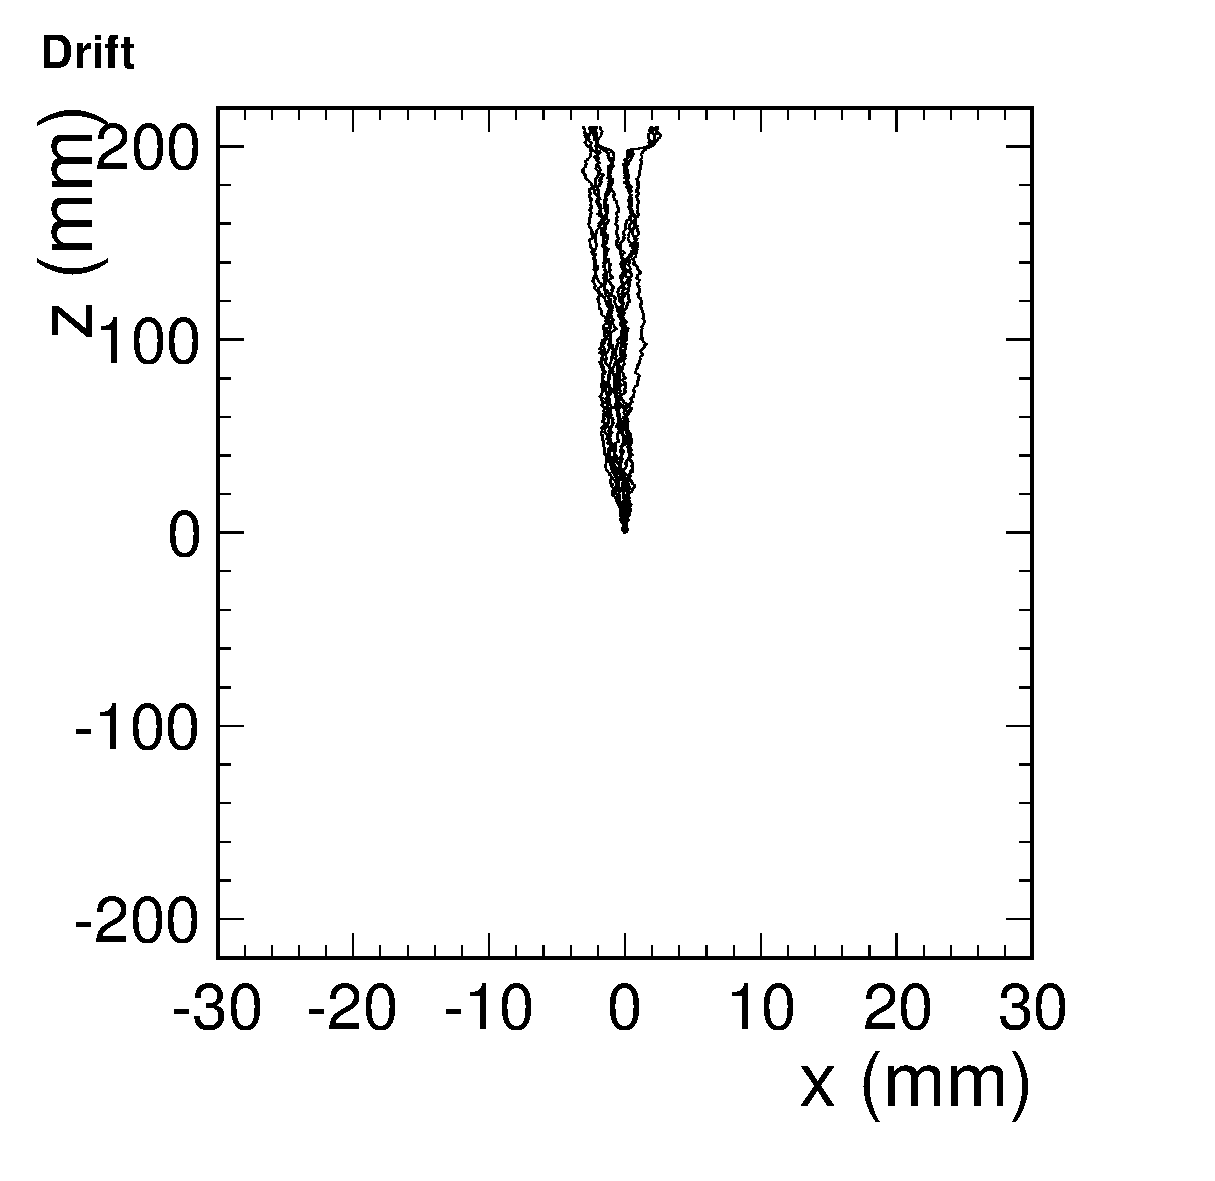
\includegraphics[width=0.3\hsize]{fig/Drift_0.eps}
%  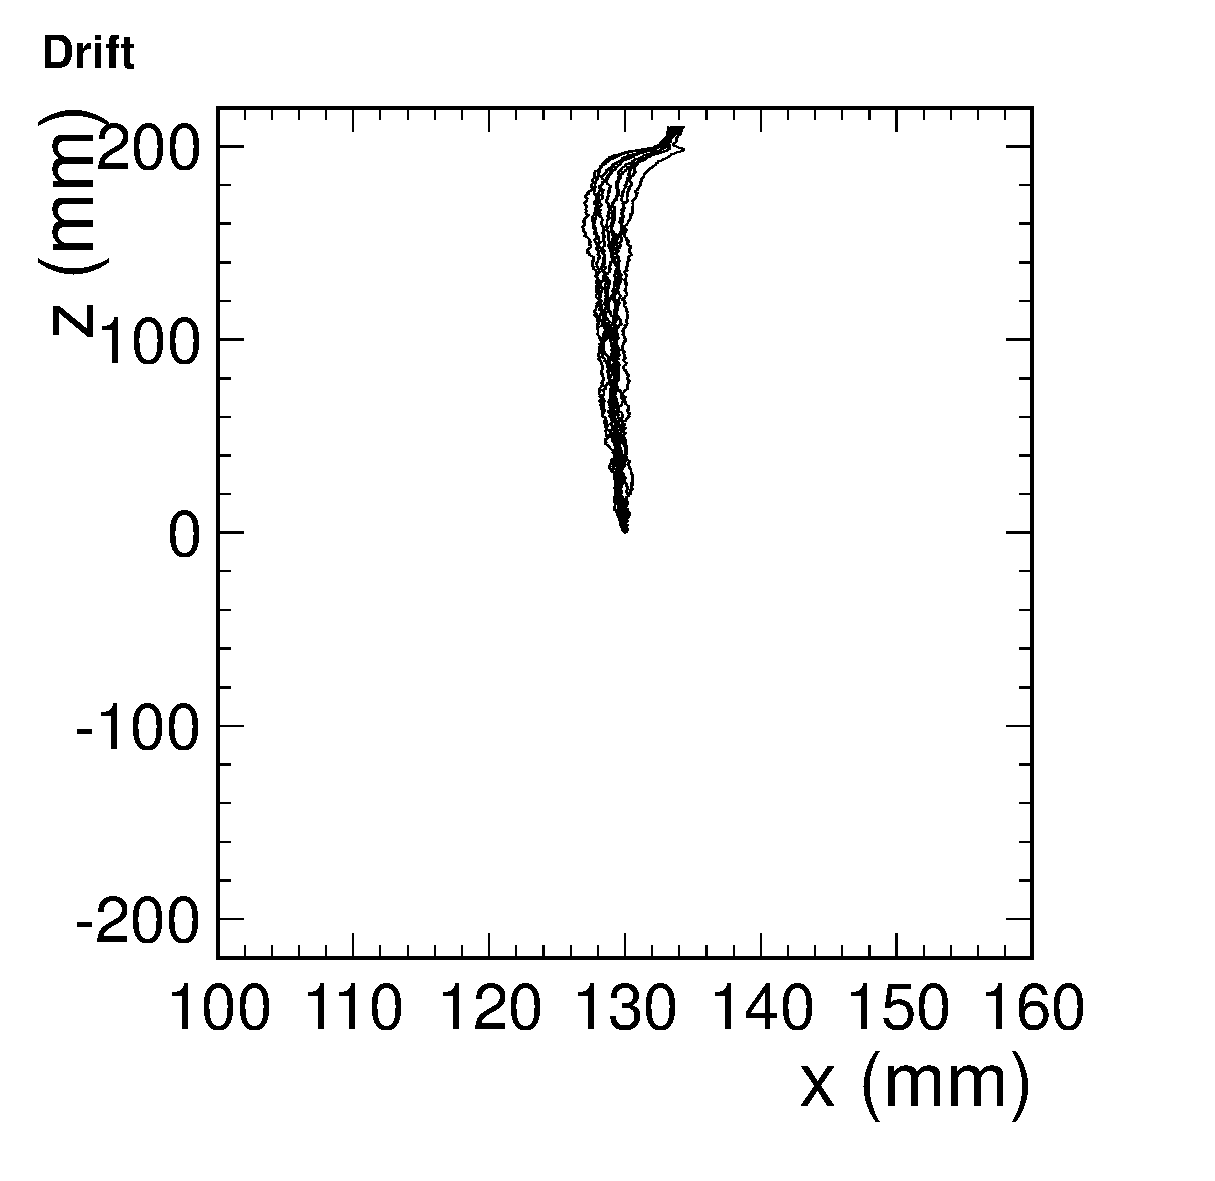
\includegraphics[width=0.3\hsize]{fig/Drift_130.eps}
%  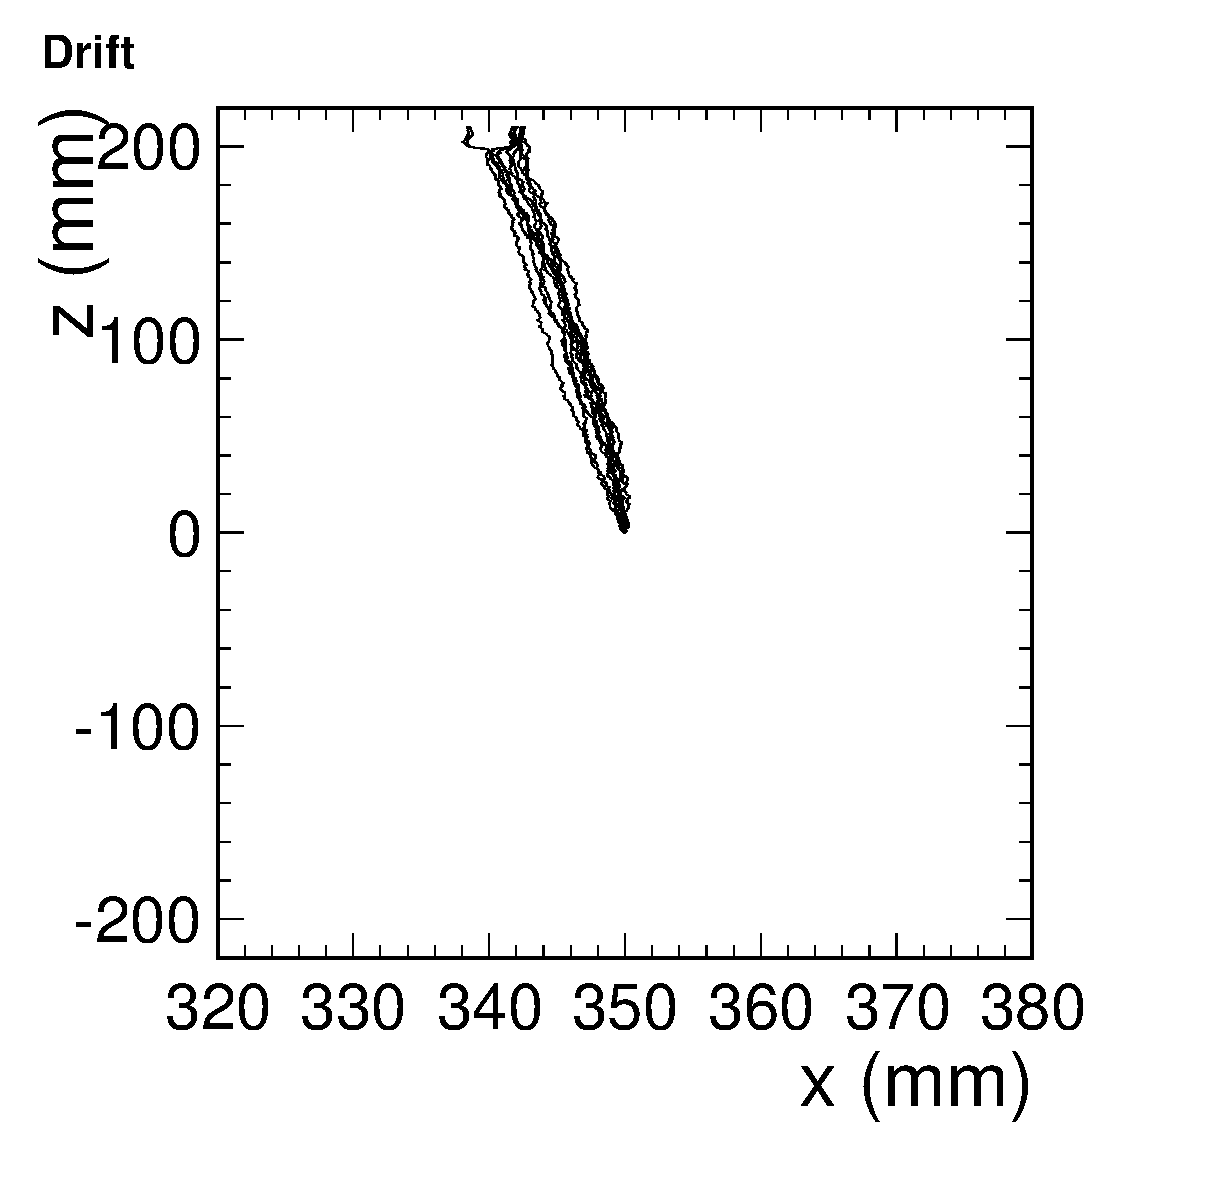
\includegraphics[width=0.3\hsize]{fig/Drift_350.eps}
% \end{center}
% \caption{Simulation of the electron drift with three different initial positions. Left, middle, and right plots corresponds to x=0, x=130 mm, and x=350 mm, respectively.}
% \label{Fig:DriftSimulation}
%\end{figure}

%\begin{itemize}
%\item Plot: drift simulation  (Tanaka)
%\end{itemize}
%\subsection{Preamp Response and Digitization}
%\begin{itemize}
%\item Preamp gain vs channel number  (Naito)
%\end{itemize}

%\subsection{FFT Noise}
%\subsection{FFT Noise}
There are two kind of noise in the data we obtained, random noise and coherent noise.
Random noise is the noise which exists in each anode channel.
Coherent noise is in each board.
The pseudo noise we implemented in Monte Carlo simulation is composed of random and coherent noise by this reason.

Random noise is generated from FFT(Fast Fourier Transform) distribution of real data. Figure \ref{example10ch} shows an example of FFT distribution.

Coherent noise is generated board by board as the noise scale in the real data we obtained.
The noise scale is defined as a root mean square of pedestal, minimun noise scale is about 3 and maximum noise scale is about 10 in the data.

The ratio of random and coherent noise is 1:1 as equation \ref{PseudoNoise}.
Figure \ref{coherentNoise} shows real data noise and pseudo noise we implemeted in Monte Carlo simulation.
\begin{equation}
  Pseudo\,Noise = \frac{Random\,Noise + Coherent\,Noise}{2}
  \label{PseudoNoise}
\end{equation}

\begin{figure}[!htb]
  \centering
  \centering
  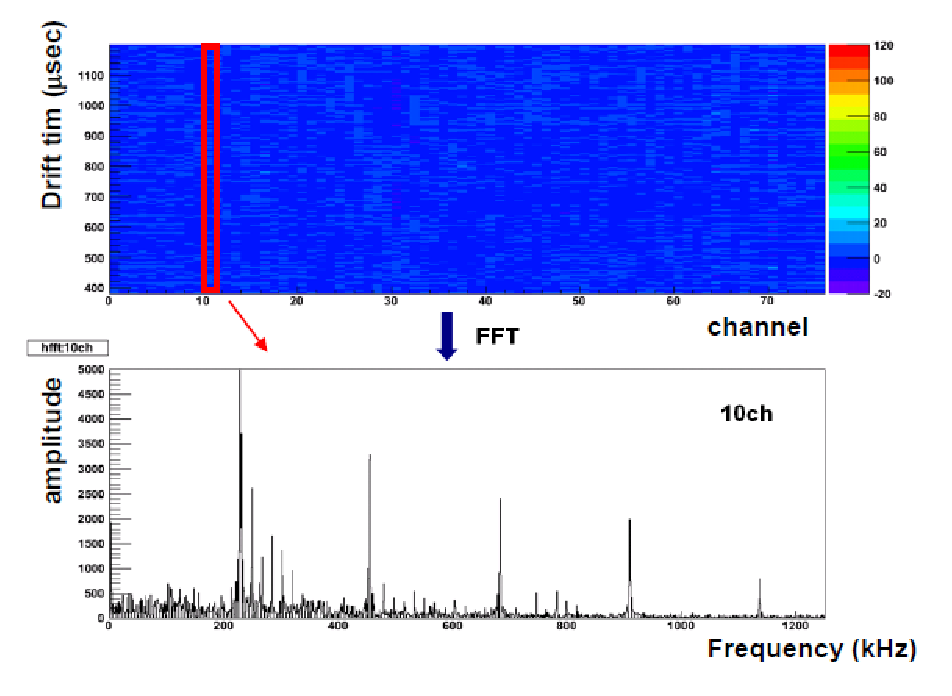
\includegraphics[width=7cm,clip]{./fig/example10ch.eps}
  \caption{example distribution of frequency:10ch}
  \label{example10ch}
\end{figure}
%\begin{figure}[!htb]
%  \centering
%  \centering
%  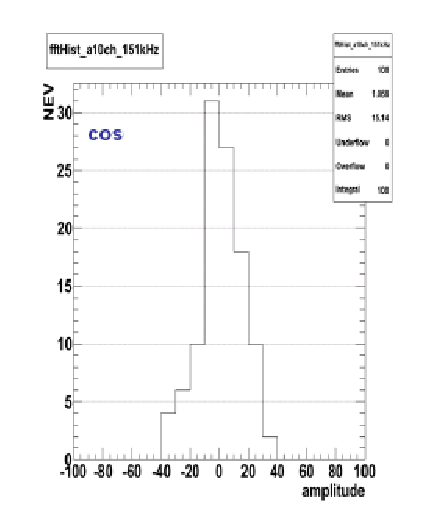
\includegraphics[width=11cm,clip]{./fig/cos.eps}
%  \caption{An example of distribution of amplitude}
%  \label{ampDist}
%\end{figure}
%\begin{figure}[!htb]
%  \centering
%  \centering
%  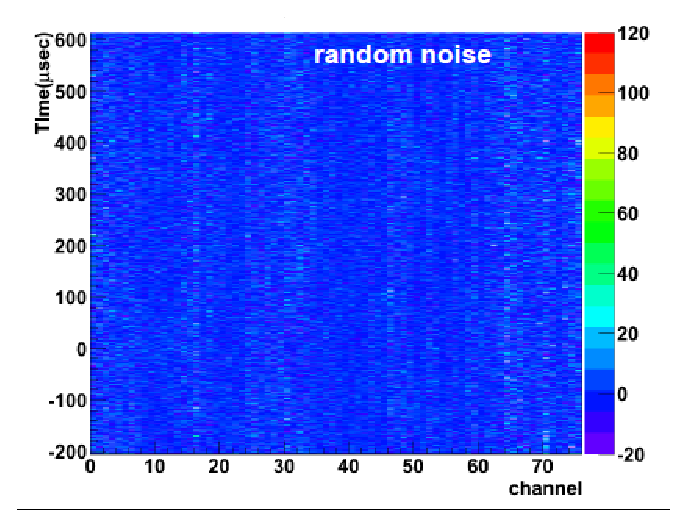
\includegraphics[width=11cm,clip]{./fig/randomnoise.eps}
%  \caption{Random noise}
%  \label{randomNoise}
%\end{figure}
\begin{figure}[!htb]
  \centering
  \centering
  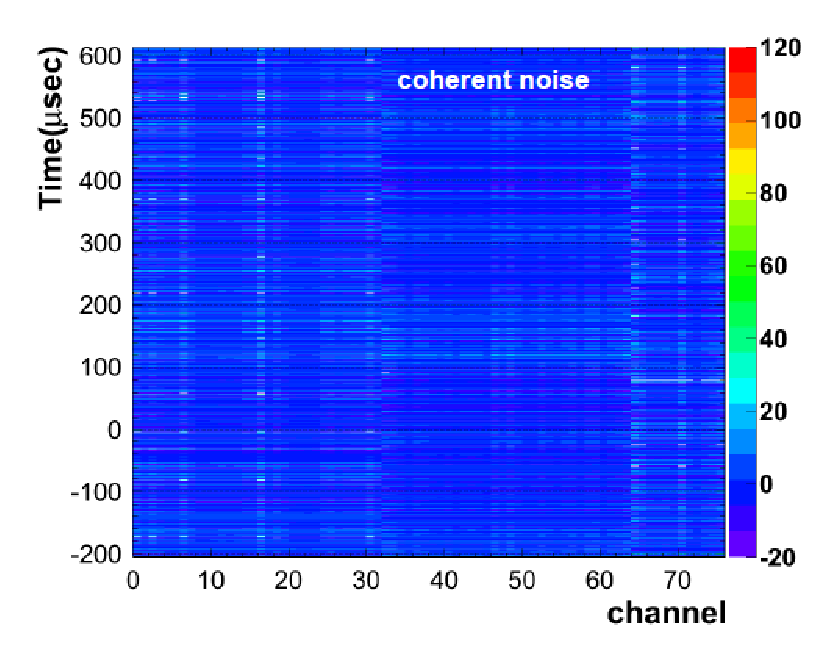
\includegraphics[width=7cm,clip]{./fig/coherentNoise.eps}
  \caption{Coherent noise}
  \label{coherentNoise}
\end{figure}
%\begin{figure}[!htb]
%  \centering
%  \centering
%  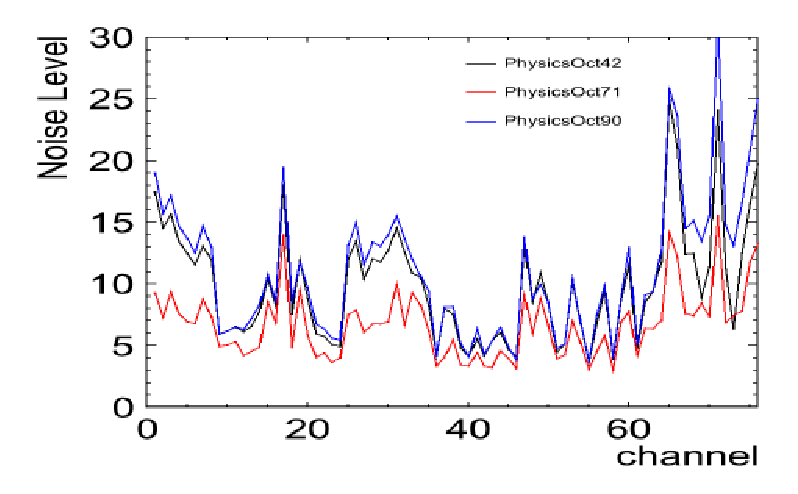
\includegraphics[width=11cm,clip]{./fig/scaling.eps}
%  \caption{Noise level}
%  \label{scaling}
%\end{figure}
\subsection{Noise Simulation}

\begin{itemize}
\item We generate noise from FFT amplitude distribution such as in Fig.\ref{Fig:FFT}
\item By using empty event, prepare template distribution of amplitude for each channel and each frequency bin
\item Obtain waveform by generating random number from the template
\item Coherent noise is added board by board
\end{itemize}

%There are two kinds of noise in the data we obtained, random noise and coherent noise.
%Random noise is the noise which exists in each anode channel.
%Coherent noise is in each board.
%The pseudo noise we implemented in Monte Carlo simulation is composed of random and coherent noise by this reason.

%Random noise is generated from FFT distribution of real data (See Fig.\ref{fig:FFT}).

%Coherent noise is generated board by board as the noise scale in the real data we obtained.
%The noise scale is defined as a root mean square of pedestal, minimum noise scale is about 3 and maximum noise scale is about 10 in the data.

%The ratio of random and coherent noise is 1:1 as equation \ref{PseudoNoise}.
%Figure \ref{DATAnoise} shows real data noise and Fig.\ref{MCnoise} shows pseudo noise we implemented in Monte Carlo simulation.
%\begin{equation}
%  Pseudo\,Noise = \frac{Random\,Noise + Coherent\,Noise}{2}
%  \label{PseudoNoise}
%\end{equation}

%\begin{figure}[!htb]
%  \centering
%  \centering
%  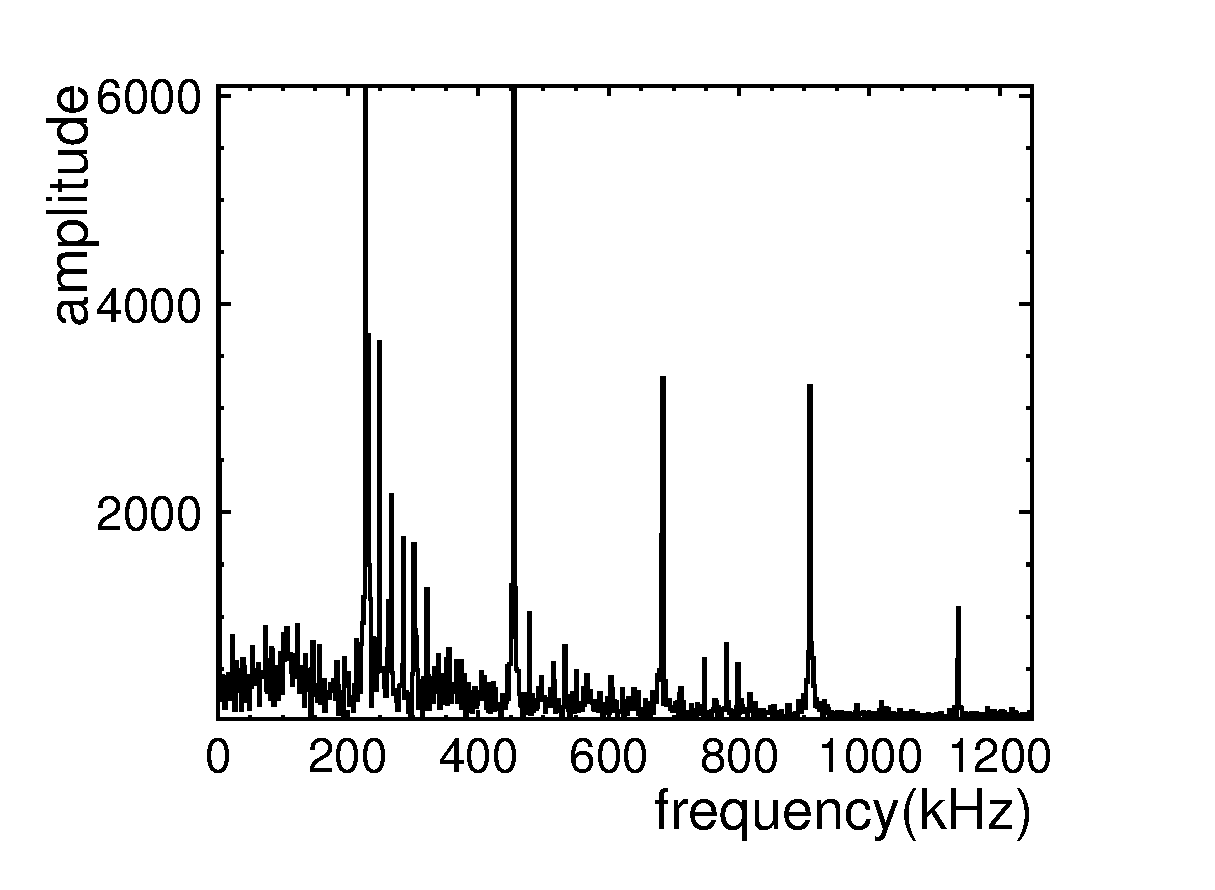
\includegraphics[width=10cm,clip]{./fig/FFTdist.eps}
%  \caption{An example distribution of frequency}
%  \label{example10ch}
%\end{figure}
%\begin{figure}[!htb]
%  \centering
%  \centering
%  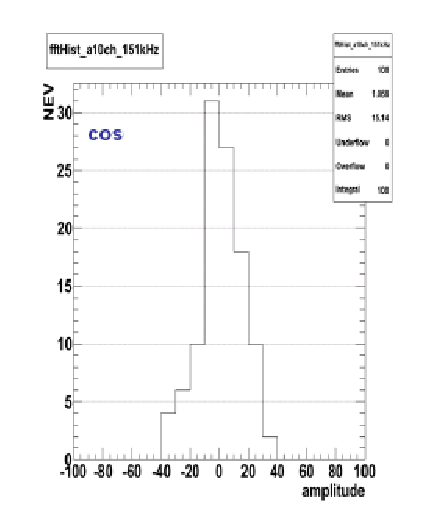
\includegraphics[width=11cm,clip]{./fig/cos.eps}
%  \caption{An example of distribution of amplitude}
%  \label{ampDist}
%\end{figure}
%\begin{figure}[!htb]
%  \centering
%  \centering
%  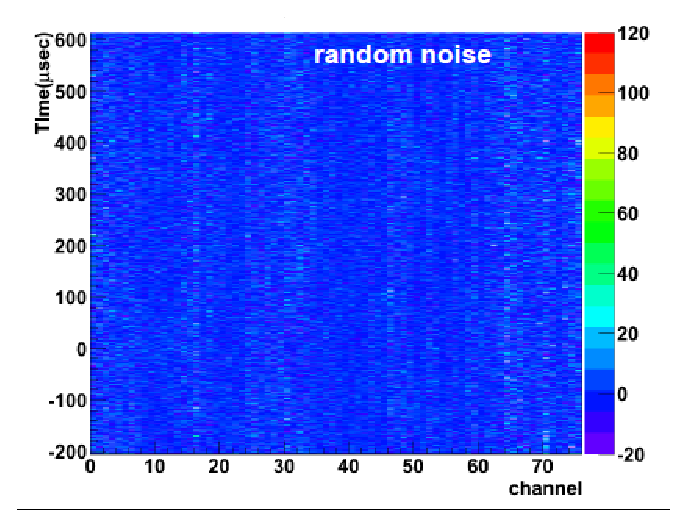
\includegraphics[width=11cm,clip]{./fig/randomnoise.eps}
%  \caption{Random noise}
%  \label{randomNoise}
%\end{figure}
%\begin{figure}[!htb]
%  \begin{center}
%    \includegraphics[width=0.45\hsize,clip]{./fig/DATAnoise.eps}
%    \includegraphics[width=0.45\hsize,clip]{./fig/MCnoise.eps}
%  \end{center}
%  \caption{Noise}
%  \label{DATAnoise}
%  \label{MCnoise}
%\end{figure}
%\begin{figure}[!htb]
%  \centering
%  \centering
%  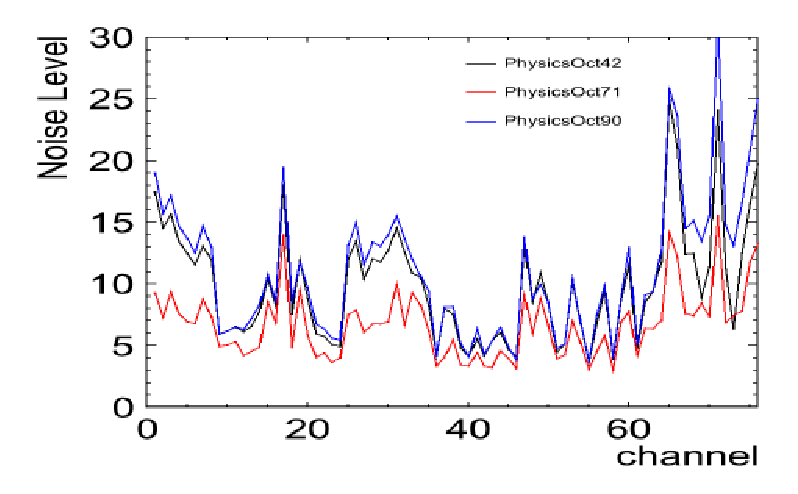
\includegraphics[width=11cm,clip]{./fig/scaling.eps}
%  \caption{Noise level}
%  \label{scaling}
%\end{figure}

Figure~\ref{Fig:SimulatedKaon} shows simulated event of 630 MeV/$c$ $K^+\to\mu\nu$.

\begin{figure}[htbp]
 \begin{center}
  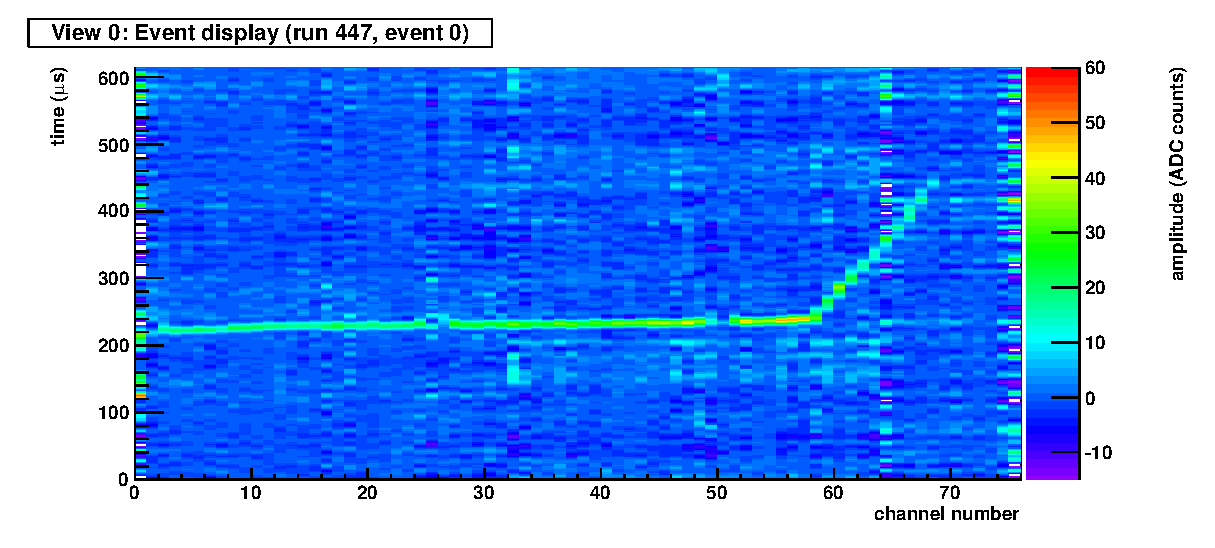
\includegraphics[width=0.8\hsize]{fig/Simulation.eps}
 \end{center}
 \caption{Event display of simulated events for 630 MeV/$c$ $K^+$.}
 \label{Fig:SimulatedKaon}
\end{figure}


%\subsection{Beam energy}
We estimated a beam momentum using simple MC simulation.
Figure \ref{K11Br_Beam_line} shows MC simulation's geometry.
We generate 800MeV/$c$ pencil beam and shoot the beam downstream.
Figure \ref{k_pi_momentum} shows Kaon and Pion momentum distribution
using this MC simulation at BDC.
Kaon beam momentum is estimated by the momentum distribution of MC simulation.
%Actually, kaon momentum distribution peak is adjusted so that kaon decay point of MC simulation is consistent with data.
%Section \ref{kaon_energy_section} explains this point.
%And proton momentum is estimated in other way, using TREK detector TOF information.
%Section \ref{proton_energy_section} shows proton momentum distribution.

\begin{figure}[!htb]
  \centering
  \centering
  \includegraphics[width=10cm,clip]{./fig/K11Br_beamline_sim.eps}
  \caption{K1.1 Br beam line}
  \label{K11Br_Beam_line}
\end{figure}


\begin{figure}[!htb]
  \centering
  \centering
  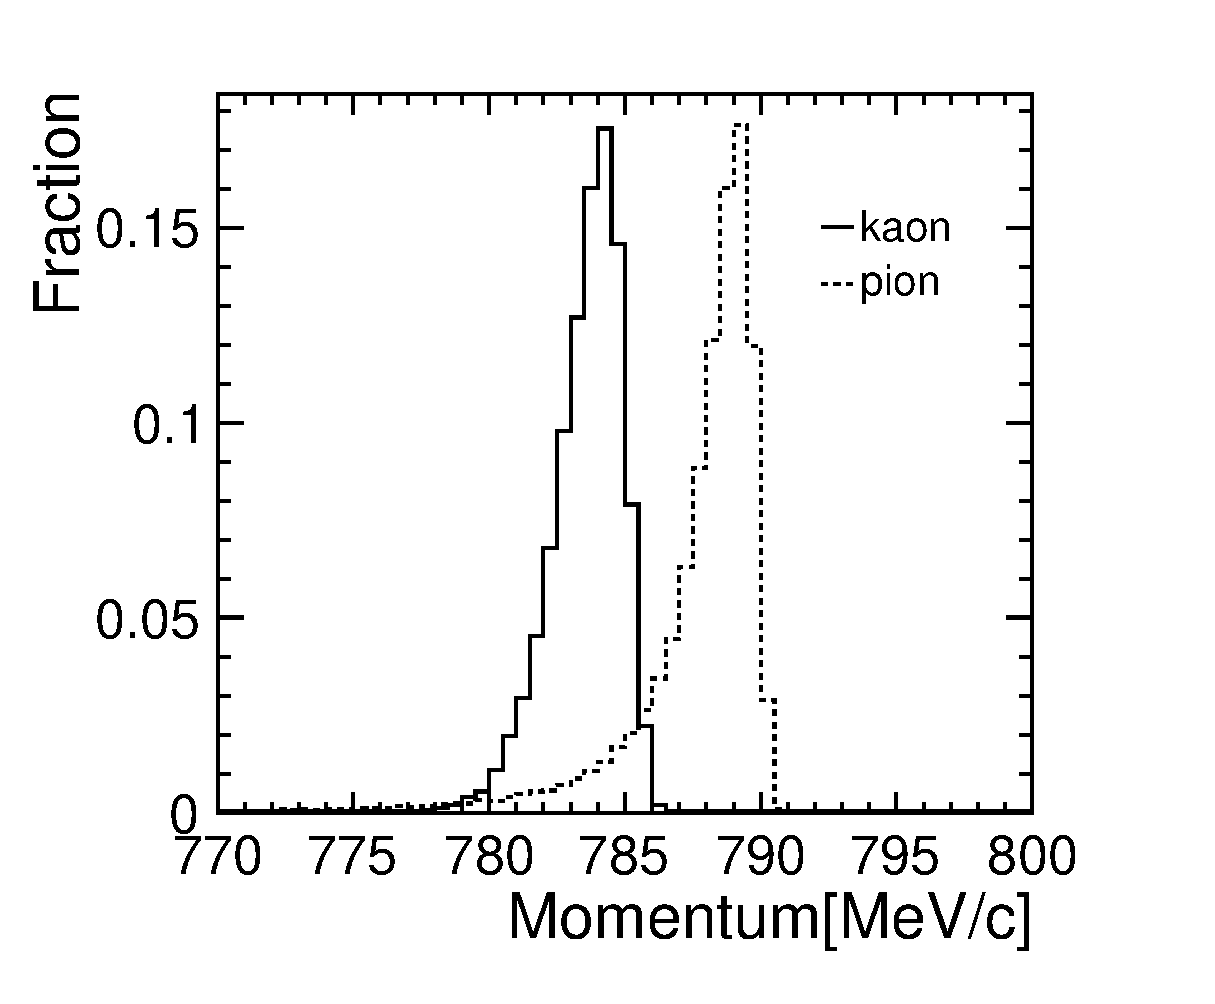
\includegraphics[width=10cm,clip]{./fig/Kaon_pion_momentum_nogrid.eps}
  \caption{Kaon and Pion momentum distribution at BDC}
  \label{k_pi_momentum}
\end{figure}


\subsubsection{Kaon energy
  \label{KaonEnergy}
}
Kaon beam momentum is estimated by the momentum distribution of MC simulation.
We change Kaon beam momentum in a range of 700 - 800 MeV/$c$ and search the momentum that decay point distribution of MC simulation is consistent with data one.

\subsubsection{Proton energy}
Proton momentum shown in Figure \ref{fig:Proton_momentum} is used as proton beam momentum of MC simulation.

\subsubsection{Energy deposition in degrader}
It is too high energy that Kaon beam stops in the fiducial volume of 250LAr TPC.
In order to degrade the beam momentum, some lead glass blocks and a lead brick were inserted in front of 250LAr TPC as degrader.
%We estimate energy deposition in degrader by using MC simulation.
Figure \ref{energy_deposition} shows energy deposition distribution in degrader.


\begin{figure}[!htb]
  \centering
  \centering
  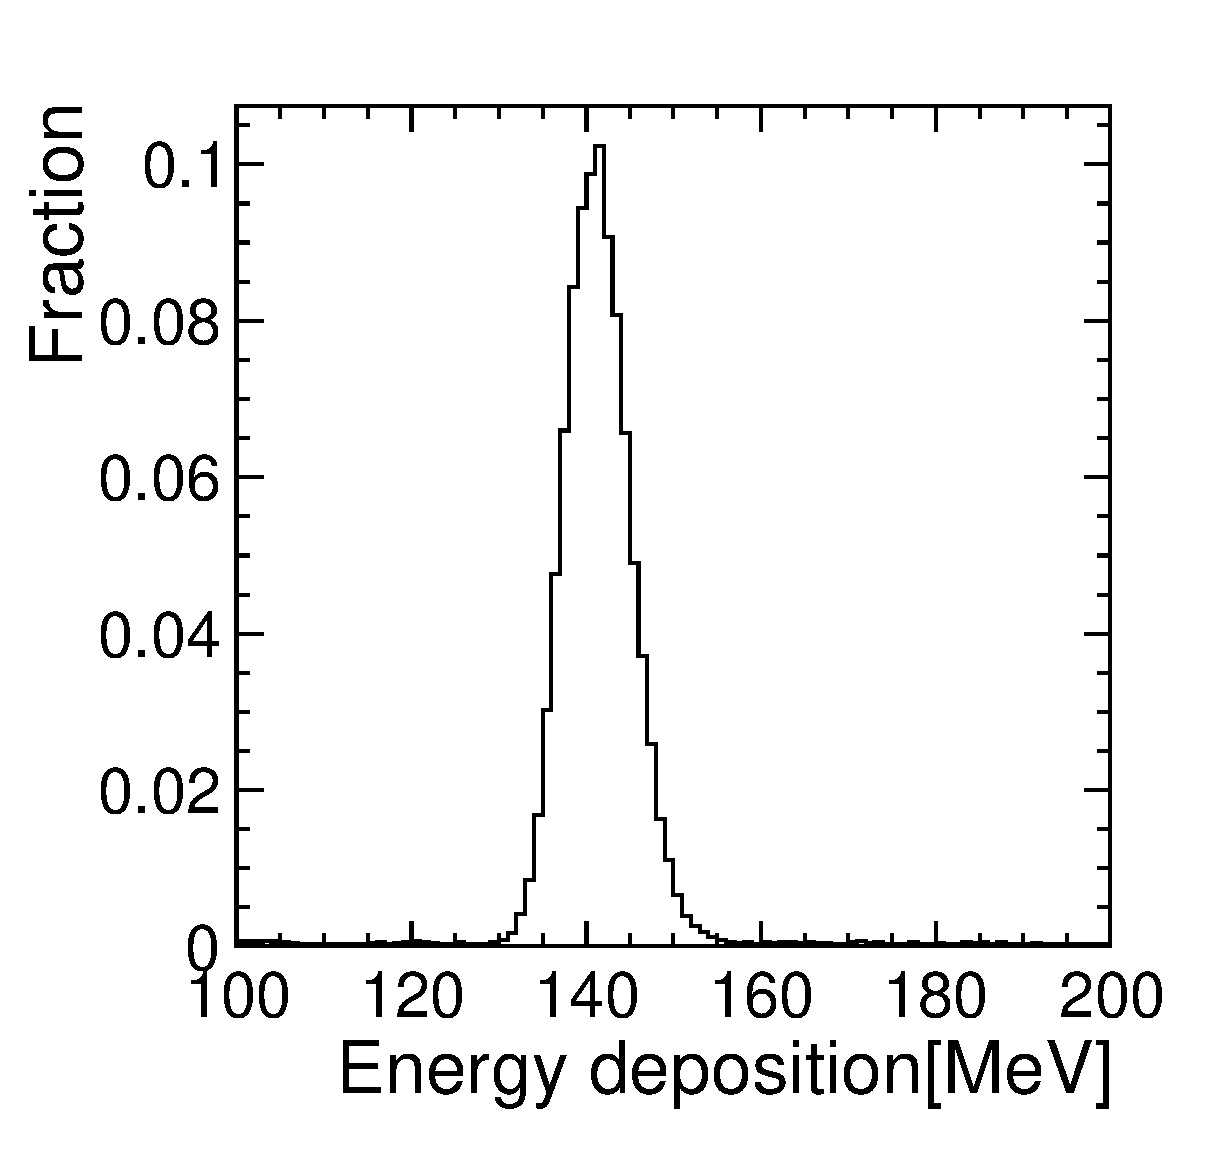
\includegraphics[width=10cm,clip]{./fig/energy_deposition.eps}
  \caption{Energy deposition in degrader}
  \label{energy_deposition}
\end{figure}





